\subsection{Data}

This analysis is performed using data from $pp$ collisions provided from the Large Hadron Collider with $\sqrt{s} = 13$~\TeV~between 2015--2018, and collected with the ATLAS detector. The total integrated luminosity of this dataset following the application of the GoodRunsList is 139~fb$^{-1}\pm1.7\%$ [GRL Ref]. The specific GoodRunsList files used are:

\begin{itemize}
    \item For 2015 data:

    data15\_13TeV/20170619/data15\_13TeV.periodAllYear\_DetStatus-v89-pro21-02\_Unknown\_PHYS\_\\
    StandardGRL\_All\_Good\_25ns.xml
    \item For 2016 data:

    data16\_13TeV/20180129/data16\_13TeV.periodAllYear\_DetStatus-v89-pro21-01\_DQDefects-00-02-04\_PHYS\_StandardGRL\_All\_Good\_25ns.xml
    \item For 2017 data:

    data17\_13TeV/20180619/data17\_13TeV.periodAllYear\_DetStatus-v99-pro22-01\_Unknown\_PHYS\_ \\
    StandardGRL\_All\_Good\_25ns\_Triggerno17e33prim.xml
    \item For 2018 data:

    data18\_13TeV/20190318/data18\_13TeV.periodAllYear\_DetStatus-v102-pro22-04\_Unknown\_PHYS\_ \\
    StandardGRL\_All\_Good\_25ns\_Triggerno17e33prim.xml
\end{itemize}

The GRID datasets used are outlined in Appendix~\ref{app:datasets}.

\subsection{Data Stability}
To check stability of data used for this analysis, rate for each year is calculated by dividing events to their corresponding luminosities. Luminosity per run is combined until summed up luminosities become either 2 fb$^{-1}$ or greater than this. Figure~\ref{fig:DataStability} depicts rate for year 2015 to 2018, where each time-ordered data bin contains 2 fb$^{-1}$ luminosity. The first bin shows rate for year 2015, bins 2--16 are for year 2016, bins 17--37 and 38--64 represent rate for year 2017 and 2018 respectively. Further, to consider those residual runs having combined luminosities smaller than 2 fb$^{-1}$, the last bin for each year is merged with the previous bin. The calculated average rate for year 2015--2018 is 2845 $\pm$ 4 and shows consistentency for each year. Figure~\ref{fig:DataStability} shows the stability of data for each year used in this analysis.
\begin{figure}[h!]
\centering
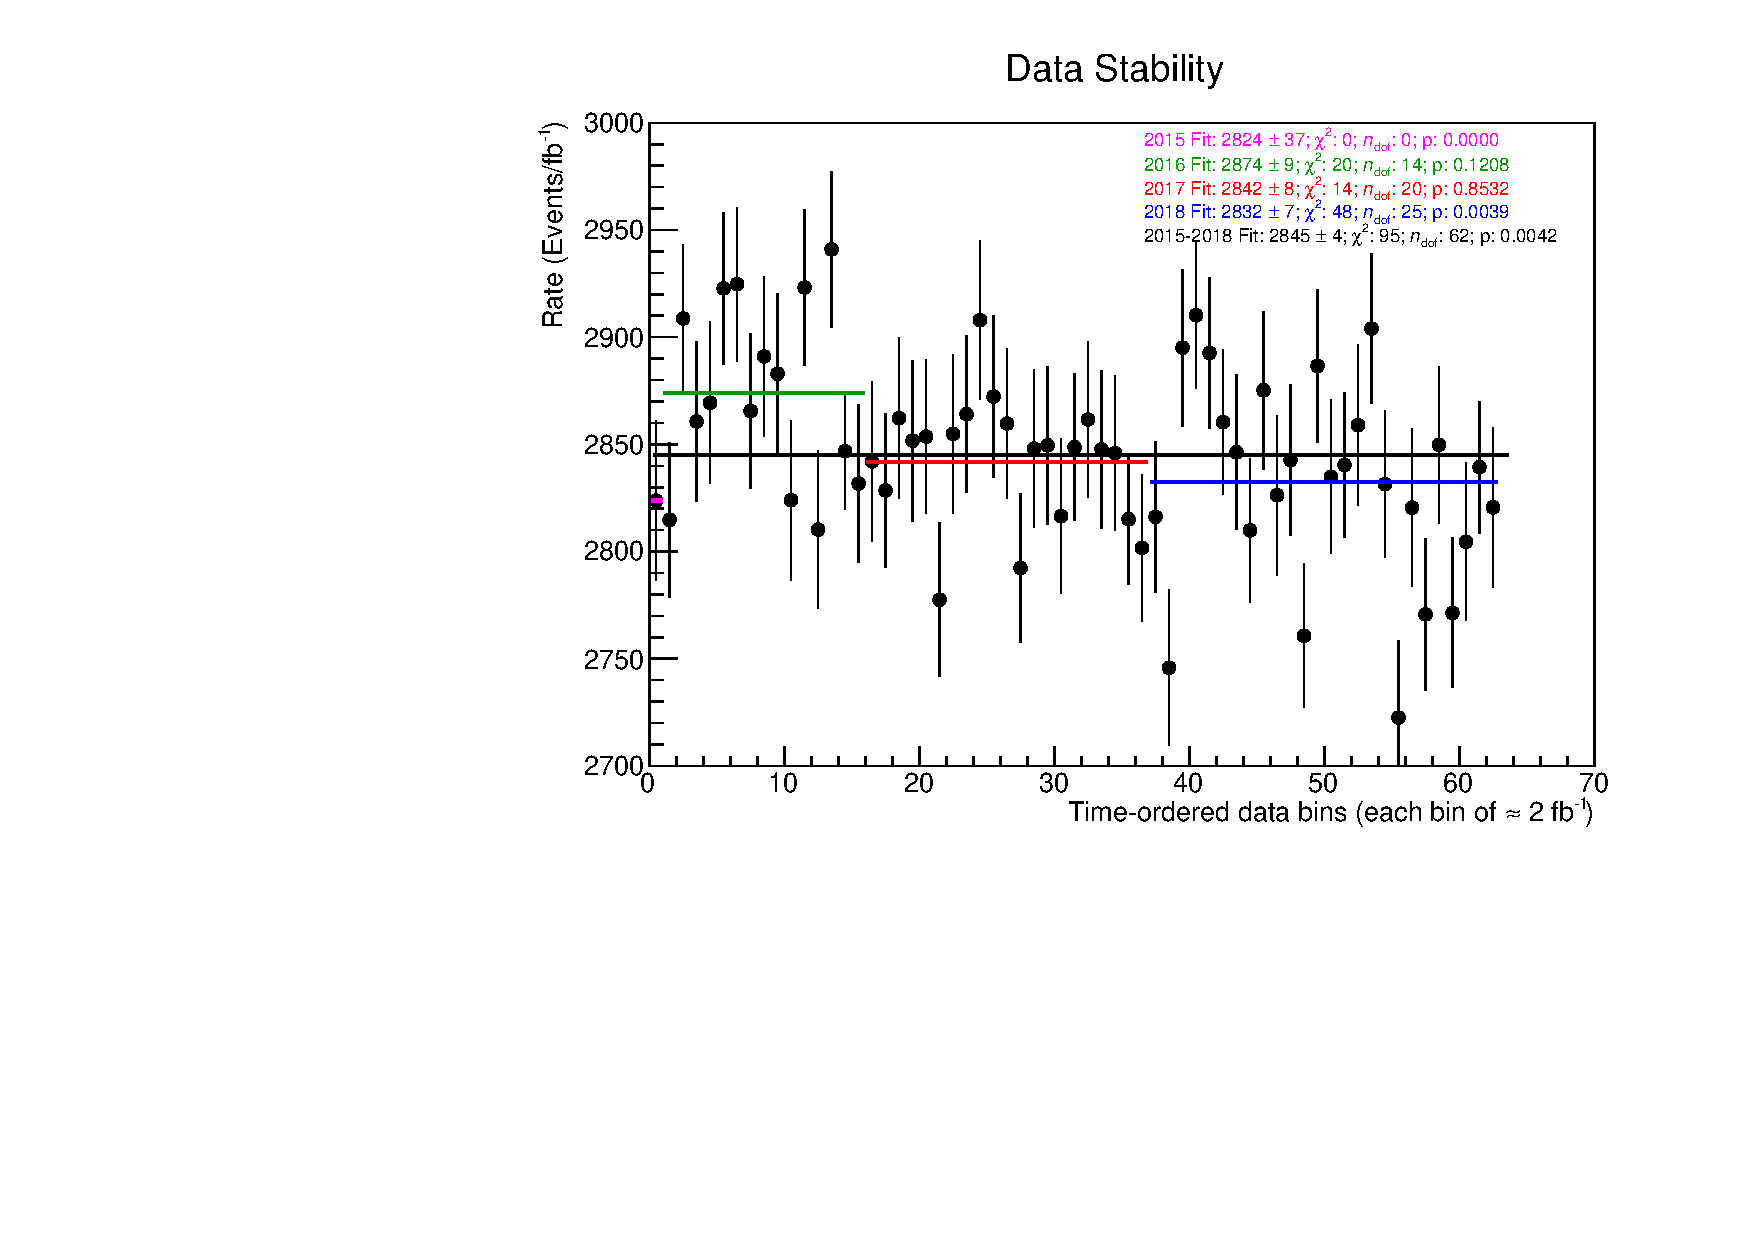
\includegraphics[width=0.75\textwidth]{figures/DataStability.pdf}
\caption{Events per fb$^{-1}$ for year 2015 to 2018, where each time-ordered data bin contains 2 fb$^{-1}$ luminosity.}
\label{fig:DataStability}
\end{figure}

\subsection{Simulation}
Monte Carlo samples can be used to compare results from data with SM predictions. The events obtained from MC samples are also used in the OmniFold method as a part of the unfolding process, which is outlined in detail in Section~\ref{subsec:omnifold}.
Due to differing pileup and detector conditions, MC samples are divided up into different campaigns: with MC16a corresponding to data taken in 2015 and 2016, MC16d to data taken in 2017, and MC16e to data taken in 2018. The analysis is performed independently
on these three campaigns and scaled according to the luminosity in order to compare the results directly with data.

Two different MC $Z\rightarrow\mu\mu$ samples are used in this analysis. The first uses Powheg-Box [Powheg references] to produces parton level events at next-to-leading order (NLO) in QCD using the CT10nlo parton distribution function (PDF), the parton level events are
then passed to Pythia 8 [Pythia Ref] which performs showering, hadronization and the subsequent particle decays.
The second dataset uses Sherpa version 2.2.1 with the NNPDF3.0 NNLO PDF to both generate and hadronize events. The Sherpa samples are accurate up to NNLO in QCD. More...

The detector response is determined by inputting the resulting events into GEANT4 simulation for the ATLAS detector [GEANT4 ref]...

The GRID datasets are listed in Appendix~\ref{app:datasets}.



